\begin{problem}{\textbf{\textsc{Trượt điện}}} 
Xem xét một khí gồm các hạt nhỏ, mỗi hạt có điện tích \( q \), bên trong một buồng hình cầu với bán kính $R$. và tâm tại gốc tọa độ. Một trường điện đều $E\hat{\mathbf{x}}$ được áp dụng bên trong buồng. Trường điện được điều chỉnh cho đến khi điểm$(R,0,0)$ có áp suất $P_0$ và tại điểm $(-R,0,0)$ có áp suất $P_0/2$ (ở trạng thái cân bằng). 

Điện trường được giảm nhanh chóng về không và khí đạt đến trạng thái cân bằng một lần nữa. Nếu áp suất cuối cùng trong buồng là $P_1$, tìm tỷ lệ $P_1/P_0$. Bỏ qua các tương tác giữa các hạt và giả sử rằng nhiệt độ của khí vẫn gần như không thay đổi.
\vspace{-0.5cm}
\begin{center}
    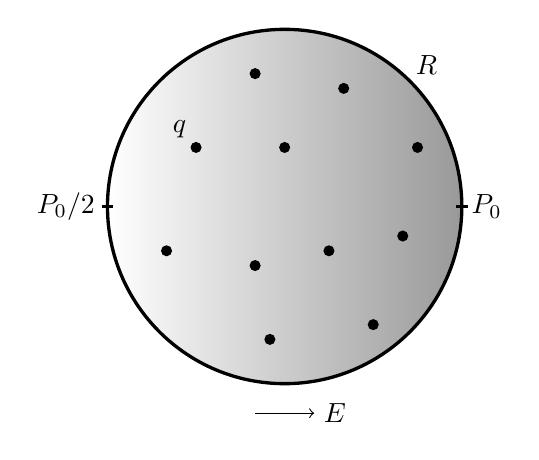
\begin{tikzpicture}[scale = 0.75, dot/.style = {circle, fill, minimum size=#1, inner sep=0pt, outer sep=0pt}]
    \draw[very thick,left color=white, right color = white!60!black] (0, 0) circle (3);
    \draw[very thick] (2.9,0)--(3.1,0);
    \node at (3, 0) [right]{$P_0$};
    \draw[very thick] (-3.1,0)--(-2.9,0);
    \node at (-3.05,0) [left]{$P_0/2$};
    \node at (2,-0.5) [dot=4]{};
    \node at (-0.5, -1) [dot=4]{};
    \node at (1, 2) [dot=4]{};
    \node at (0, 1)[dot=4]{};
    \node at (0.75, -0.75)[dot=4]{};
    \node at (-2, -0.75)[dot=4]{};
    \node at (-1.5, 1) [dot=4]{};
    \node at (1.5, -2) [dot=4]{};
    \node at (-0.5, 2.25) [dot=4]{};
    \node at (-0.25, -2.25) [dot=4]{};
    \node at (2.25, 1) [dot=4]{};
    \node at (-1.5, 1) [above left]{$q$};
    \node at (2.4, 2.4) {$R$};
    \draw [->] (-0.5, -3.5) -- (0.5, -3.5) node[right]{$E$};
    \end{tikzpicture}
\end{center}
\end{problem}
